\documentclass{jfm}
\usepackage{graphicx}
\usepackage{amsmath,amssymb,bm}
\usepackage{booktabs}

\newcommand{\Uvec}{\mathbf{U}}
\newcommand{\Uinf}{\mathbf{U}_\infty}
\newcommand{\dd}{\mathrm{d}}
\newcommand{\rhoinf}{\rho_\infty}
\newcommand{\pinf}{p_\infty}
\newcommand{\uinf}{u_\infty}
\newcommand{\xv}{\bm{x}}
\newcommand{\Aann}{\mathcal{A}}

\shorttitle{Far-field boundary conditions for compressible IBM flow}
\shortauthor{J. Qiao}

\title{Far-field boundary conditions for an immersed-boundary
compressible solver: reflection, mean-state anchoring, and a
drift-free aeroacoustic metric}

\author{J. Qiao\aff{1}
  \corresp{\email{qiaojiaye970122@gmail.com}}}

\affiliation{\aff{1}Cerisse compressible immersed-boundary solver,
validation campaign}

\begin{document}

\maketitle

\begin{abstract}
The Cerisse Cartesian-AMR immersed-boundary solver offers three usable
far-field ghost-cell closures --- zero-gradient extrapolation
(\textit{foextrap}), hard Dirichlet freestream, and an algebraic
Riemann-invariant ``NSCBC'' --- and the question of which best represents an
open boundary recurs in every external-flow validation case. We answer it with
three controlled experiments of increasing dimensionality. A one-dimensional
Poinsot--Lele acoustic-pulse benchmark shows the as-shipped algebraic closure
returns $78\%$ of a normally incident wave; we trace this exactly to the
$\sigma\!\to\!\infty$ (perfectly reflecting) limit of a relaxed
characteristic boundary condition, and a one-line correction
($J^-_{\mathrm{ghost}}=J^-_\infty$ instead of $p_{\mathrm{ghost}}=\pinf$)
restores $R<10^{-5}$ while preserving mean-state anchoring. A two-dimensional
co-rotating vortex pair then tests genuine multi-directional radiation. We
introduce a drift-free, phase-aware acoustic-corruption metric --- a per-point
least-squares single-tone phasor evaluated in a far-field annulus and
referenced to a reflection-free wide-domain truth, with a
truth-against-itself noise floor --- and find that \textit{every} closure's
corruption of the radiated quadrupole lies below the measurement floor: the
free-radiation wave does not discriminate the boundary conditions. The single
field that does separate them is the mean pressure (the DC mode). Finally, a
supersonic cylinder demonstrates where the characteristic closure is decisive:
when an oblique bow shock crosses a near lateral boundary, the corrected
characteristic condition enables a $2.5\times$ domain reduction with the shock
stand-off preserved to $7\%$, whereas \textit{foextrap} catastrophically
destroys the upstream field. Boundary-condition quality for compressible
external flow is therefore governed by mean-state anchoring and shock crossing,
not by free-wave reflection.
\end{abstract}

\begin{keywords}
computational methods, shock waves, aeroacoustics
\end{keywords}

\section{Introduction}\label{sec:intro}
The Cerisse solver is a block-structured Cartesian adaptive-mesh-refinement
(AMR) code for the compressible Navier--Stokes equations with an image-point
immersed-boundary method (IBM); it uses a WENO-Z fifth-order reconstruction, an
HLLC Riemann solver and a strong-stability-preserving Runge--Kutta integrator.
Its external-flow validation suite --- a cylinder at $M=1.7$, spheres at $M=2$
and $M=4$ --- prescribes a supersonic Dirichlet inflow on the upstream face and
one of several closures on the remaining (lateral and downstream) faces. A
schlieren A/B comparison on the cylinder showed visible differences in the
lateral far field, raising a question that this paper settles: \emph{which
far-field boundary condition (BC) best represents an open boundary for
compressible external flow, and why?}

The literature on non-reflecting boundaries is mature. \citet{thompson1987} cast
the Euler equations in characteristic form at boundaries; \citet{poinsot1992}
extended this to the Navier--Stokes characteristic boundary condition (NSCBC)
with a linear-relaxation closure for the incoming wave, building on the
acoustically non-reflecting analysis of \citet{rudy1980}. Multidimensional
corrections that account for transverse and viscous terms were added by
\citet{yoo2007} and \citet{lodato2008}. \citet{colonius2004} reviews the field,
including absorbing (sponge) layers. Crucially, \citet{motheau2017} showed that
a \emph{ghost-cell} NSCBC --- the only kind expressible in a finite-volume AMR
code that fills ghost cells once per stage --- is a legitimate and modern
formulation, not a compromise.

Against this backdrop we report three findings. First
(\S\S\ref{sec:closures}--\ref{sec:1d}), a 1-D benchmark diagnoses why the
solver's algebraic ``NSCBC'' reflected, and a corrected characteristic closure
is verified non-reflecting. Second (\S\S\ref{sec:cvp}--\ref{sec:cvpresults}), a
2-D co-rotating vortex pair, analysed with a new drift-free aeroacoustic metric,
shows that for free radiation no closure beats simple extrapolation on the wave.
Third (\S\ref{sec:cylinder}), a supersonic cylinder identifies the regime ---
oblique strong-shock crossing --- where the characteristic closure is genuinely
and dramatically superior. Throughout, quantities are non-dimensionalised by a
reference density, sound speed and length.

\section{The far-field closures}\label{sec:closures}
Let $\bm n$ be the outward unit normal and $\Uvec=(\rho,\rho\bm u,\rho E)^\top$
the conservative state. Cerisse fills ghost cells through a user
\texttt{bcnormal} routine; the integer codes \texttt{1} (ext\_dir),
\texttt{2} (foextrap) and \texttt{7} (ext\_dir, characteristic) select the
closures below. With $u_n=\bm u\!\cdot\!\bm n$ and sound speed $c$ the boundary
eigenvalues are $\{u_n-c,\,u_n,\,u_n+c\}$ and four regimes arise.

\subsection{Zero-gradient extrapolation (\textit{foextrap}, code 2)}
First-order extrapolation copies the first interior cell into every ghost layer,
\begin{equation}
\Uvec_{\mathrm{ghost}}=\Uvec_{\mathrm{int}}
\quad\Longleftrightarrow\quad
\partial\Uvec/\partial n|_{\partial\Omega}=\bm 0 .
\end{equation}
Nothing is prescribed; every characteristic is extrapolated. For a purely
outgoing disturbance the ghost is a faithful continuation, so the boundary
Riemann problem has (to first order) no jump and no reflected wave. The weakness
is that nothing anchors the boundary, so in a closed subsonic region the mean
pressure can drift, and obliquely incident waves are partially reflected.

\subsection{Hard Dirichlet freestream (code 1)}
Every ghost layer is overwritten with the constant freestream
$\Uvec_{\mathrm{ghost}}=\Uinf$. At a supersonic inflow ($M_n\le-1$) all
characteristics enter and this is exact; at a subsonic boundary it
over-specifies, clamping $\rho,\bm u$ to freestream and corrupting any outgoing
entropy or vorticity wave, and conflicting with any non-freestream mean state
(e.g.\ post-shock gas where a bow shock crosses the boundary).

\subsection{Algebraic Riemann-invariant closure (``NSCBC'', code 7)}
\label{sec:alg}
The ghost is built from a local characteristic analysis. For the subsonic
outflow branch $0\le u_n<c$ the outgoing invariant $J^+=u_n+2c/(\gamma-1)$ and
the entropy $s=p/\rho^\gamma$ are taken from the interior, and the single
incoming acoustic characteristic must be fixed. The as-shipped closure
\emph{hard-imposed the back-pressure},
\begin{equation}
\boxed{\,p_{\mathrm{ghost}}=\pinf\,},\qquad \rho,\bm u,s\ \text{from interior}.
\label{eq:pin}
\end{equation}
This is the standard steady-state external-aerodynamics far-field: at
convergence of a steady flow no waves reach the boundary and it is exact. For
\emph{unsteady} waves, however, \eqref{eq:pin} is reflective, as \S\ref{sec:1d}
shows.

\subsection{Reference: relaxed Poinsot--Lele NSCBC}
The proper NSCBC does not pin the pressure. The outgoing amplitudes are computed
from interior one-sided differences and the single incoming amplitude
$\mathcal L_1$ is \emph{relaxed} toward the target,
\begin{equation}
\mathcal L_1=\sigma\,(1-M^2)\,\frac{c}{L}\,(p-\pinf),
\label{eq:relax}
\end{equation}
with $\sigma\approx0.25$ and $L$ a reference length, after which the boundary
state evolves by the LODI relations
\begin{equation}
\frac{\partial p}{\partial t}=-\tfrac12(\mathcal L_5+\mathcal L_1),\quad
\frac{\partial u_n}{\partial t}=-\tfrac1{2\rho c}(\mathcal L_5-\mathcal L_1).
\end{equation}
The limit $\sigma\!\to\!0$ is perfectly non-reflecting but lets $p$ drift;
$\sigma\!\to\!\infty$ forces $p=\pinf$ instantly and is perfectly reflecting ---
i.e.\ \eqref{eq:pin}.

\section{One-dimensional reflection benchmark}\label{sec:1d}
We solve the 1-D Euler equations with the same HLLC solver Cerisse uses
(first-order Godunov, $N=1000$, $L=10$, $c_0=1$). A right-running acoustic pulse
$\delta p=A\exp[-((x-x_0)/w)^2]$ with $\delta u=\delta p/(\rho_0c_0)$,
$\delta\rho=\delta p/c_0^2$ is launched toward the outflow boundary in a uniform
mean flow of normal Mach number $M_n$. The ghost BCs are filled exactly as in
the solver; the reference \eqref{eq:relax} replaces the boundary-cell
right-hand side by the LODI update. The energy-based reflection coefficient
$R=\max_t|\delta p_{\mathrm{ref}}|/\max_t|\delta p_{\mathrm{inc}}|$ is measured
at an interior sensor.

\begin{figure}
  \centering
  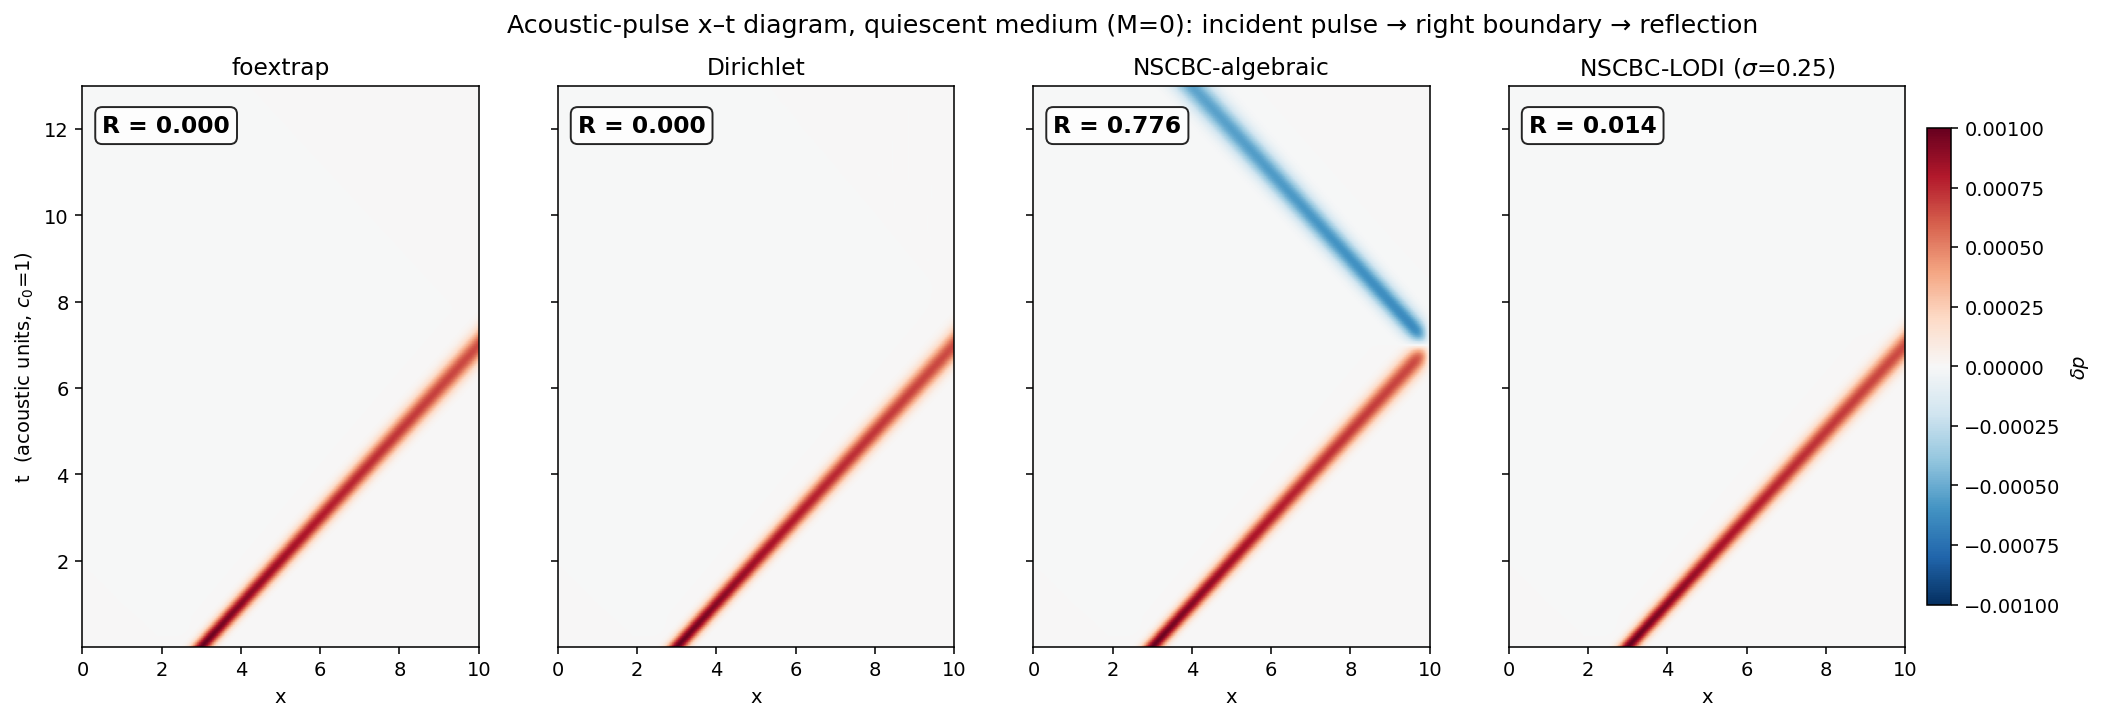
\includegraphics[width=\textwidth]{figures/xt_diagrams_M0.png}
  \caption{Acoustic-pulse $x$--$t$ diagrams at $M=0$. The incident pulse travels
  up-and-right; a returning (up-and-left) streak is a reflection. Only the
  as-shipped algebraic ``NSCBC'' \eqref{eq:pin} produces one;
  \textit{foextrap}, hard Dirichlet and the relaxed reference let the pulse
  leave cleanly.}
  \label{fig:xt}
\end{figure}

\subsection{Reflection at a quiescent boundary}
Figure~\ref{fig:xt} shows the $x$--$t$ evolution. Table~\ref{tab:R0} lists $R$
at $M=0$: the algebraic closure returns $R=0.78$, while \textit{foextrap},
Dirichlet and the relaxed NSCBC are non-reflecting. A separate entropy-advection
test produced zero spurious pressure for all closures, confirming the
differences are purely acoustic.

\begin{table}
  \centering
  \begin{tabular}{lcccc}
    & \textit{foextrap} & Dirichlet & NSCBC-algebraic & NSCBC-LODI ($\sigma{=}0.25$)\\[3pt]
    $R$ at $M=0$ & $5\times10^{-6}$ & $2\times10^{-6}$ & $\mathbf{0.776}$ & $0.014$\\
    mean-drift residual & $1.00$ & $0.50$ & $\mathbf{0.00}$ & $0.65$\\
  \end{tabular}
  \caption{Reflection coefficient and mean-anchoring residual ($1=$ no
  anchoring) at a quiescent boundary. No simple ghost closure achieves both low
  reflection and tight anchoring; the trade-off is intrinsic.}
  \label{tab:R0}
\end{table}

\subsection{Root cause and correction}
Figure~\ref{fig:root} sweeps the relaxation $\sigma$ of the reference
\eqref{eq:relax} at $M=0.1$. At $\sigma=0$ the reference is non-reflecting; at
the recommended $\sigma=0.25$, $R=0.011$; and as $\sigma\to\infty$ the
reflection rises monotonically to $R=0.674$ at $\sigma=200$, converging onto the
algebraic value $R=0.693$ (dashed). \emph{The algebraic closure is numerically
the $\sigma\to\infty$ limit of a relaxed NSCBC}: it hard-pins $p=\pinf$
\eqref{eq:pin} instead of relaxing toward it. This is a design choice (a fixed
back-pressure outflow), not a coding error.

\begin{figure}
  \centering
  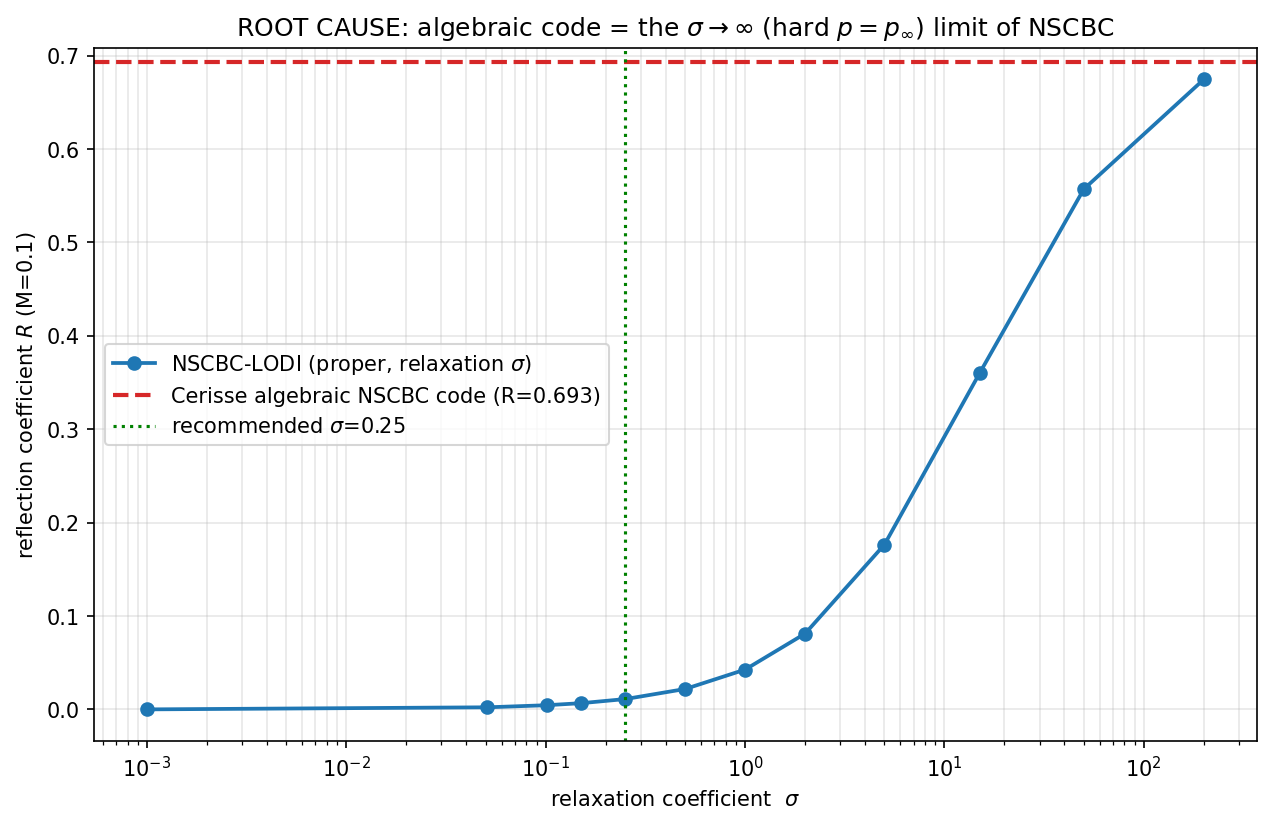
\includegraphics[width=0.8\textwidth]{figures/root_cause_sigma.png}
  \caption{Root cause: reflection of the relaxed reference NSCBC versus its
  relaxation $\sigma$ at $M=0.1$. The dashed line is the as-shipped algebraic
  closure; it coincides with $\sigma\to\infty$.}
  \label{fig:root}
\end{figure}

The correction follows directly. Rather than pinning the pressure, the
subsonic-outflow branch sets the \emph{incoming} Riemann invariant to its
freestream value while keeping the outgoing invariant and entropy from the
interior,
\begin{equation}
J^-_{\mathrm{ghost}}=J^-_\infty=u_{n,\infty}-\frac{2c_\infty}{\gamma-1},\quad
J^+_{\mathrm{ghost}}=J^+_{\mathrm{int}},\quad
s_{\mathrm{ghost}}=s_{\mathrm{int}},
\label{eq:fix}
\end{equation}
the textbook Thompson/Whitfield characteristic non-reflecting outflow. In the
1-D test this drops $R$ from $0.78$ to below $10^{-5}$ at $M=0$, while retaining
the anchoring of the incoming invariant to the freestream that \textit{foextrap}
lacks. All subsequent ``characteristic'' (code 7) runs use \eqref{eq:fix}.

\subsection{The reflection--anchoring trade-off}
Figure~\ref{fig:drift} starts the domain at a uniform over-pressure and asks
whether each closure relaxes the box back to $\pinf$. \textit{foextrap}
prescribes nothing, so it never anchors (residual $1.00$); the algebraic pin
anchors perfectly and fastest (residual $0.00$) but that same pin reflects; the
relaxed NSCBC sits between. The reflectivity of the algebraic closure is the
price of its perfect mean-anchoring (Table~\ref{tab:R0}). This tension ---
reflection versus anchoring --- is the thread that the 2-D and shock tests
resolve.

\begin{figure}
  \centering
  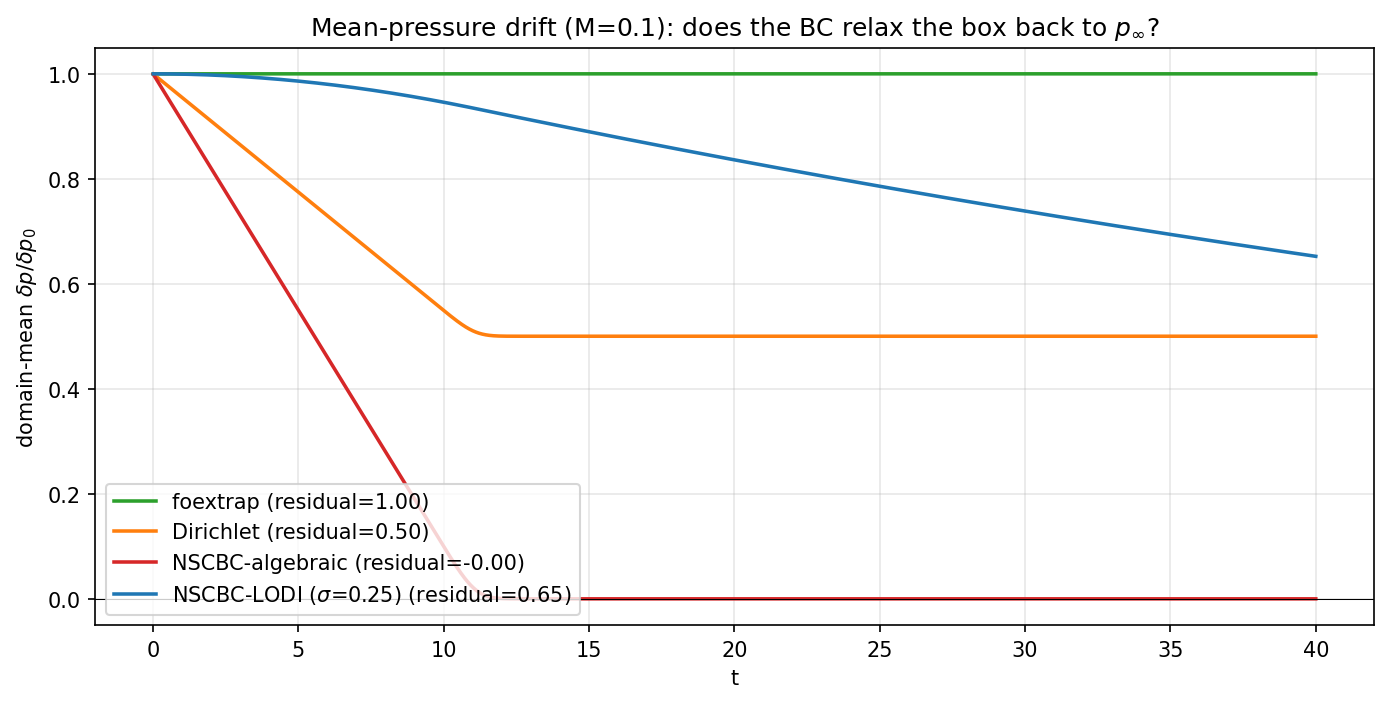
\includegraphics[width=0.8\textwidth]{figures/pressure_drift.png}
  \caption{Mean-pressure relaxation from an initial over-pressure, $M=0.1$.
  \textit{foextrap} never returns to $\pinf$; the algebraic pin returns fastest.
  Anchoring and non-reflection are in tension.}
  \label{fig:drift}
\end{figure}

\section{A two-dimensional aeroacoustic test: the co-rotating vortex
pair}\label{sec:cvp}
The 1-D benchmark isolates normal-incidence reflection. A far-field BC for
aeroacoustics must also pass an obliquely radiating, multi-directional wave
without corrupting it. We use the canonical model source: the sound radiated by
a co-rotating vortex pair \citep{mitchell1995}, solved with the production
solver (2-D, WENO-Z, inviscid Euler, no IBM).

\subsection{Problem and initial condition}
Two identical Lamb--Oseen vortices of circulation $\Gamma$ and core radius $r_c$
sit at $\xv_{1,2}=(\pm b/2,0)$, each with tangential profile
\begin{equation}
u_\theta(r)=\frac{\Gamma}{2\pi r}\Big(1-e^{-r^2/r_c^2}\Big),
\end{equation}
the velocity field being their vector superposition. Being of equal sign the
pair co-rotates rigidly about the origin at
\begin{equation}
\Omega=\frac{\Gamma}{\pi b^2},\qquad
V_{\mathrm{orb}}=\tfrac12\Omega b,\qquad
M_{\mathrm{orb}}=\frac{V_{\mathrm{orb}}}{c_0}.
\end{equation}
Because the configuration is invariant under rotation by $\pi$, the far field is
a rotating lateral quadrupole ($m=2$) that radiates at \emph{twice} the orbital
frequency,
\begin{equation}
f_{\mathrm{ac}}=\frac{\Omega}{\pi}=2\cdot\frac{\Omega}{2\pi},\qquad
\lambda=\frac{c_0}{f_{\mathrm{ac}}}.
\end{equation}
We take $M_{\mathrm{orb}}=0.20$, $b=1$, $r_c=0.25$, $\gamma=1.4$, with
$\rho_0=c_0=1$ (so $p_0=1/\gamma$), giving $\Gamma=2\pi b\,c_0M_{\mathrm{orb}}
=1.257$, $\Omega=0.40$, $T_{\mathrm{rot}}=2\pi/\Omega=15.71$,
$f_{\mathrm{ac}}=0.1273$ and $\lambda=T_{\mathrm{ac}}=7.854$.

The radiated pressure is only $O(\rho_0V_{\mathrm{orb}}^4/c_0^2)\sim10^{-3}$, so
the initial state must be in \emph{compressible} radial equilibrium or the
startup transient swamps the sound. Imposing the incompressible balance
$\dd p/\dd r=\rho_0u_\theta^2/r$ together with an isentropic density is
inconsistent at $M_{\mathrm{swirl}}\sim0.5$ and launches a spurious monopole.
The consistent state satisfies, with $p=p_0(\rho/\rho_0)^\gamma$ and
$c^2=\gamma p/\rho$,
\begin{equation}
\frac{\dd p}{\dd r}=\rho\,\frac{u_\theta^2}{r}
\;\Longleftrightarrow\;
\frac{\dd c^2}{\dd r}=(\gamma-1)\frac{u_\theta^2}{r}
\;\Longrightarrow\;
c^2(r)=c_0^2-(\gamma-1)\!\int_r^\infty\!\frac{u_\theta^2(r')}{r'}\,\dd r',
\label{eq:csq}
\end{equation}
after which $\rho=\rho_0(c^2/c_0^2)^{1/(\gamma-1)}$ and
$p=p_0(c^2/c_0^2)^{\gamma/(\gamma-1)}$. The deficit integral has a closed form
in exponential integrals for the Lamb--Oseen profile; it is evaluated per vortex
and the two are superposed. This removes the startup monopole and leaves the
clean rotating-quadrupole spiral of figure~\ref{fig:spiral}, computed on a wide
$\pm40$ domain that is reflection-free over the analysis window and serves as
the reference truth.

\begin{figure}
  \centering
  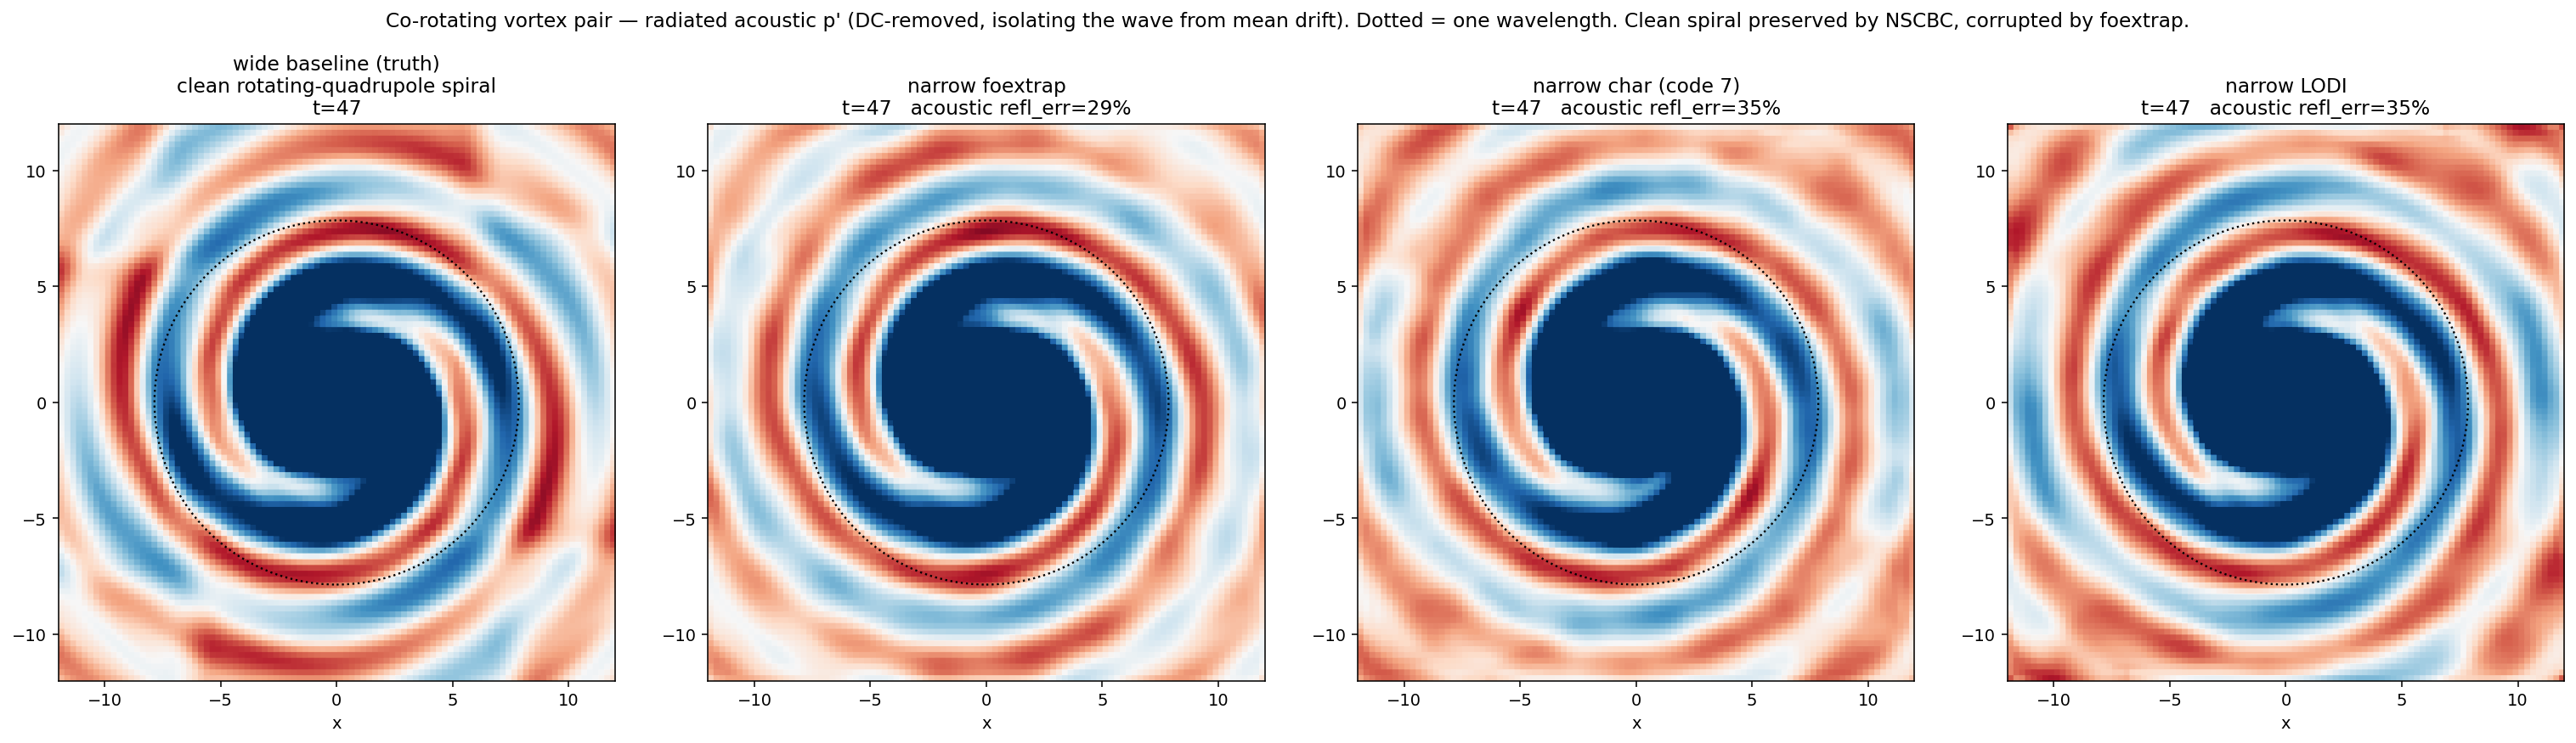
\includegraphics[width=\textwidth]{figures/cvp_acoustic_spiral.png}
  \caption{Reference (wide $\pm40$) radiated rotating-quadrupole spiral
  (pressure perturbation). This reflection-free field is the truth against which
  truncated-domain closures are measured.}
  \label{fig:spiral}
\end{figure}

\section{A drift-free, phase-aware acoustic-corruption metric}\label{sec:metric}
We quantify how much a truncated-domain closure corrupts the radiated wave with
a single dimensionless number immune to (i) mean-pressure drift, (ii)
instantaneous phase misalignment between runs, and (iii) near-field
contamination.

\subsection{Single-tone phasor by least squares}
At each point $\xv$ in a far-field annulus the pressure record over the window
$[t_0,t_1]$ is modelled as a mean, a linear drift and the acoustic fundamental,
\begin{equation}
p(\xv,t)\approx c_0(\xv)+c_3(\xv)(t-\bar t)
+c_1(\xv)\cos\omega_{\mathrm{ac}}t+c_2(\xv)\sin\omega_{\mathrm{ac}}t,
\quad\omega_{\mathrm{ac}}=2\pi f_{\mathrm{ac}},
\end{equation}
the four coefficients recovered per point by least squares on the actual
(non-uniform, CFL-limited) snapshot times $\{t_k\}$. The complex quadrupole
phasor is $\hat P(\xv)=c_1+\mathrm{i}c_2$, with
$p'\sim\mathrm{Re}\{\hat P\,e^{-\mathrm{i}\omega_{\mathrm{ac}}t}\}$.

\emph{Why least squares and not a discrete Fourier transform.} On uniform,
integer-period sampling the kernel $e^{-\mathrm{i}\omega t}$ is exactly
orthogonal to the constant and linear modes, so a single-bin DFT cleanly
extracts the tone. The solver's output times are non-uniform and the field
carries a slow, BC-dependent mean drift; off the uniform grid the kernel is not
orthogonal to $\{1,t\}$ and a naive DFT leaks the drift into the tone bin. On a
synthetic record (8\% time jitter plus DC, drift and tone) the integer-bin and
Hann-windowed DFT recover $|\hat P|$ to $\sim1\%$ but the \emph{complex} value
(its phase) by $>100\%$; the least-squares fit, carrying explicit $\{1,(t-\bar
t)\}$ columns, makes the tone orthogonal to the mean and drift for \emph{any}
sampling and recovers amplitude and phase to $1.5\%$. Neither a mean offset nor
a linear drift (an un-anchored BC) can then pollute $\hat P$.

\subsection{Drift-free broadband RMS}
As a phase-insensitive companion we detrend each point (subtract the fitted
$c_0+c_3(t-\bar t)$, not merely the mean) and form
\begin{equation}
\mathrm{RMS}(\xv)=\left(\frac1T\int_{t_0}^{t_1}
\big[p-c_0-c_3(t-\bar t)\big]^2\dd t\right)^{1/2},\quad T=t_1-t_0,
\end{equation}
the amplitude of all unsteady content. Being an amplitude it is phase-blind by
construction; detrending (not de-meaning) is essential, or a ramping mean would
survive and inflate it.

\subsection{Annulus, reference and corruption number}
Both fields are evaluated only on
$\Aann=\{\xv:R_{\mathrm{in}}\le|\xv|\le R_{\mathrm{out}}\}$,
$R_{\mathrm{in}}=9.0\approx1.15\lambda$, $R_{\mathrm{out}}=10.5$. The inner edge
keeps the whole annulus in the radiation zone (evanescent near-field terms,
decaying faster than the radiating $\sim r^{-1/2}$ part of a 2-D multipole, are
negligible); the outer edge stays $1.5$ inside the narrow $\pm12$ boundary,
clear of the truncation band. The wide $\pm40$ run is reflection-free in $\Aann$
over the window: a wave emitted near $t=0$ reaches its boundary at $t\approx40$
and re-enters $\Aann$ only at $t\approx69.5$, after the window closes
($t_1=55$). For each truncated closure the corruption is the area-weighted
annulus-$L^2$ relative error,
\begin{equation}
E_F^{\mathrm{cplx}}=\frac{\|\hat P-\hat P_{\mathrm w}\|_\Aann}{\|\hat P_{\mathrm w}\|_\Aann},\quad
E_F^{\mathrm{amp}}=\frac{\big\||\hat P|-|\hat P_{\mathrm w}|\big\|_\Aann}{\big\||\hat P_{\mathrm w}|\big\|_\Aann},\quad
E_{\mathrm{RMS}}=\frac{\|\mathrm{RMS}-\mathrm{RMS}_{\mathrm w}\|_\Aann}{\|\mathrm{RMS}_{\mathrm w}\|_\Aann},
\end{equation}
with $\|f\|_\Aann=(|\Aann|^{-1}\!\int_\Aann|f|^2\dd A)^{1/2}$ and subscript $\mathrm w$
the wide truth. The window $[t_0,t_1]$ spans an integer number of acoustic
periods ($4T_{\mathrm{ac}}=[23.6,55]$, beginning $\sim1.5\,T_{\mathrm{rot}}$
after start) so the fit is leakage-clean.

\subsection{Noise floor: the decisive honesty check}
Even the reflection-free truth is imperfectly reproducible: the source is weak
($M_{\mathrm{orb}}=0.2\Rightarrow$ radiated amplitude $\sim10^{-3}$) and the
annulus carries residual unsteady near field and discretisation noise. We
estimate the floor by a truth-against-itself test: split the wide window into
two \emph{disjoint} halves of equal integer period count ($2+2\,T_{\mathrm{ac}}$),
compute $\hat P$ and $\mathrm{RMS}$ on each, and take their annulus-$L^2$
difference. \textbf{Any corruption below this floor is not resolvable.}

\section{Results: the radiated wave is not a discriminator}\label{sec:cvpresults}
Table~\ref{tab:cvp} collects the corruption numbers for the three
truncated-domain ($\pm12$) closures --- \textit{foextrap}, corrected
characteristic \eqref{eq:fix}, and the multidimensional LODI helper with a
finite, anchoring-enabling relaxation $\sigma_p=0.25$ --- against the wide
truth.

\begin{table}
  \centering
  \begin{tabular}{lcccc}
    BC (narrow $\pm12$) & $E_F^{\mathrm{amp}}$ (\%) & $E_F^{\mathrm{cplx}}$ (\%)
      & $E_{\mathrm{RMS}}$ (\%) & mean drift\\[3pt]
    \textit{foextrap} (code 2)       & $53.7$ & $70.3$ & $4.8$  & $-8.2\times10^{-5}$\\
    characteristic (code 7)          & $49.8$ & $85.1$ & $5.8$  & $+1.4\times10^{-4}$\\
    LODI ($\sigma_p{=}0.25$)         & $65.4$ & $96.3$ & $10.0$ & $+7.2\times10^{-3}$\\[3pt]
    \textbf{noise floor} (truth split)& $\mathbf{64.1}$ & --- & $\mathbf{14.4}$ & ---\\
    wide ($\pm40$, truth)            & $0$ & $0$ & $0$ & $4.2\times10^{-4}$\\
  \end{tabular}
  \caption{Acoustic-corruption numbers (annulus-$L^2$ versus the wide truth,
  drift-free, phase-aware, $4T_{\mathrm{ac}}$ window). Every closure's wave
  corruption lies \emph{at or below} the truth-against-itself noise floor
  ($64\%$ Fourier, $14\%$ RMS): the radiated wave does not discriminate the
  closures. Only the DC mean drift separates them, where \textit{foextrap} and
  characteristic anchor ($\sim10^{-4}$) while the finite-relaxation LODI drifts
  $50\times$ more.}
  \label{tab:cvp}
\end{table}

\subsection{The wave is below the floor}
For every closure the Fourier-tone corruption ($50$--$65\%$) is at or below the
$64\%$ truth-against-itself floor, and the drift-free broadband RMS corruption
($5$--$10\%$) is below the $14\%$ floor. The radiated quadrupole at
$M_{\mathrm{orb}}=0.2$ is too weak, and the annulus too contaminated by the
rotating-spiral near field, to resolve any closure's effect on the wave. The
large Fourier floor is the phase-$L^2$ sensitivity of a rotating spiral --- its
arms have many near-zero crossings, so a small phase shift produces a large
relative $L^2$. Indeed the four $|\hat P|$ panels (figure~\ref{fig:phat}) are
visually near-identical spirals, and the $r=9$ directivity
(figure~\ref{fig:dir}) is a noisy, BC-independent trace rather than a clean
$\cos2\theta$ lobe pattern. The floor does \emph{not} shrink with window length
(it is set by the source's own non-stationarity), so a longer run cannot lift
the signal above it: the radiated-wave reflection is definitively not a
discriminator for these closures in this case.

\begin{figure}
  \centering
  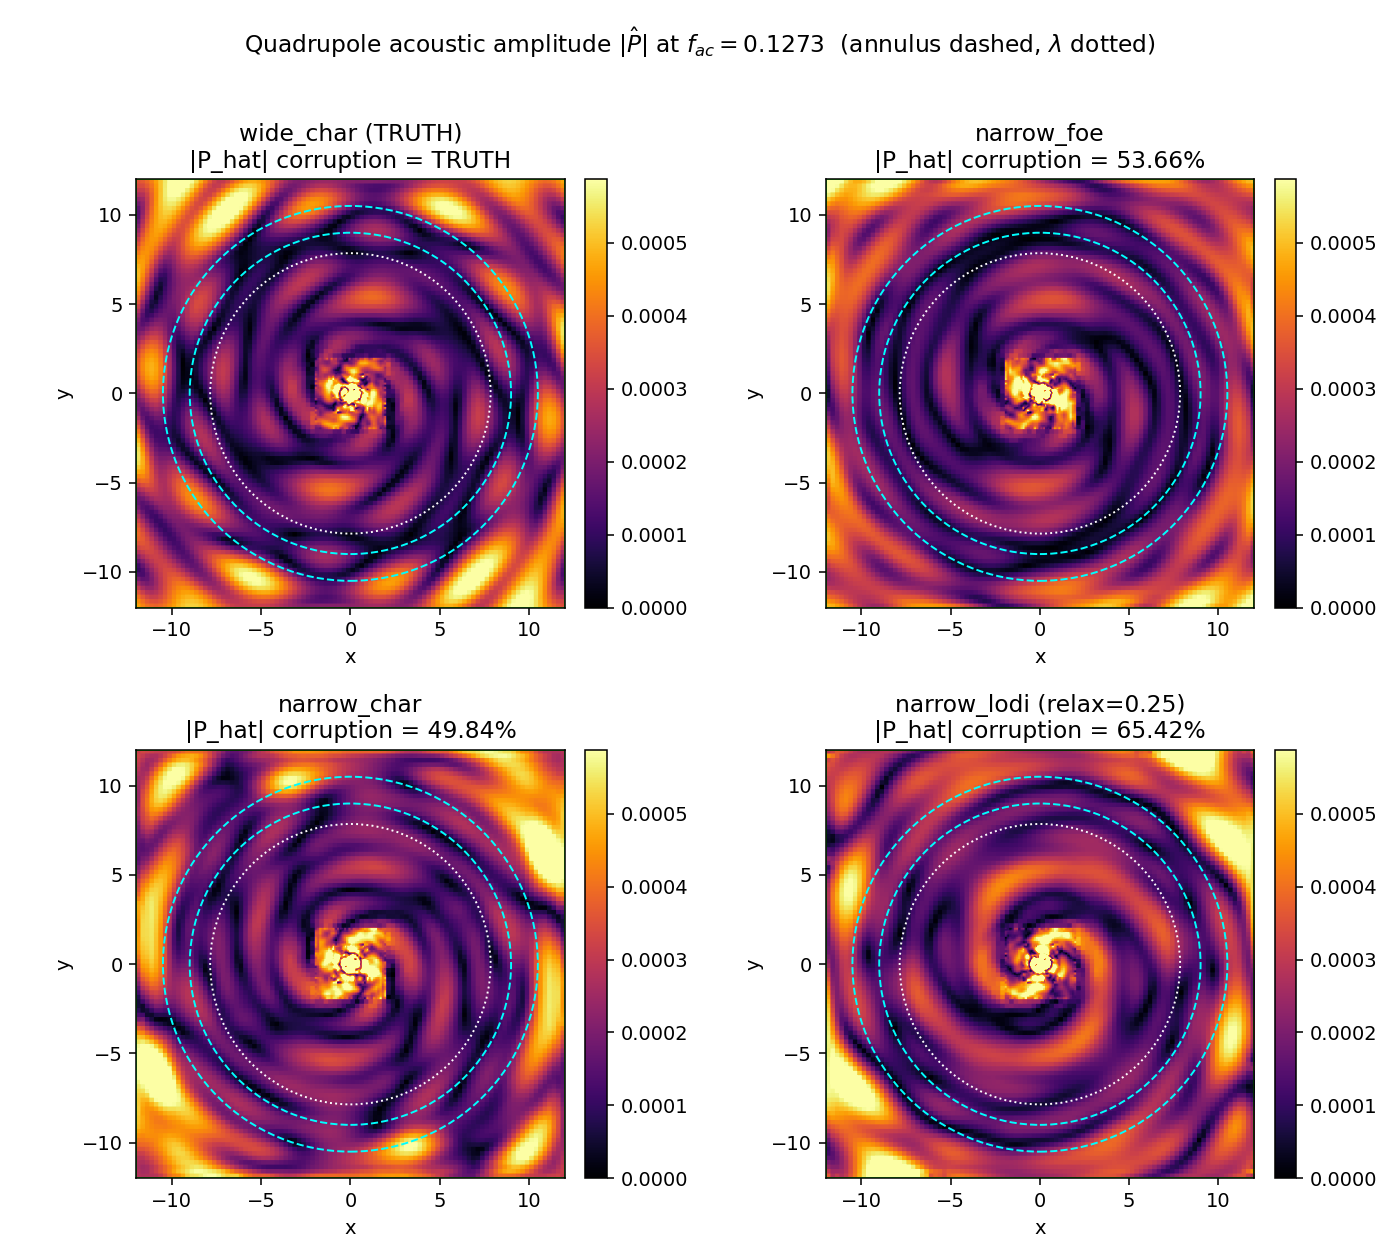
\includegraphics[width=0.8\textwidth]{figures/cvp_pHat_quadrupole.png}
  \caption{Quadrupole acoustic amplitude $|\hat P|$ at $f_{\mathrm{ac}}=0.1273$
  for the four runs (annulus dashed, $\lambda$ dotted). Truth and the three
  truncated-domain closures are visually near-identical spirals; quoted
  percentages are the annulus-$L^2$ amplitude corruptions, all near the $64\%$
  noise floor.}
  \label{fig:phat}
\end{figure}

\begin{figure}
  \centering
  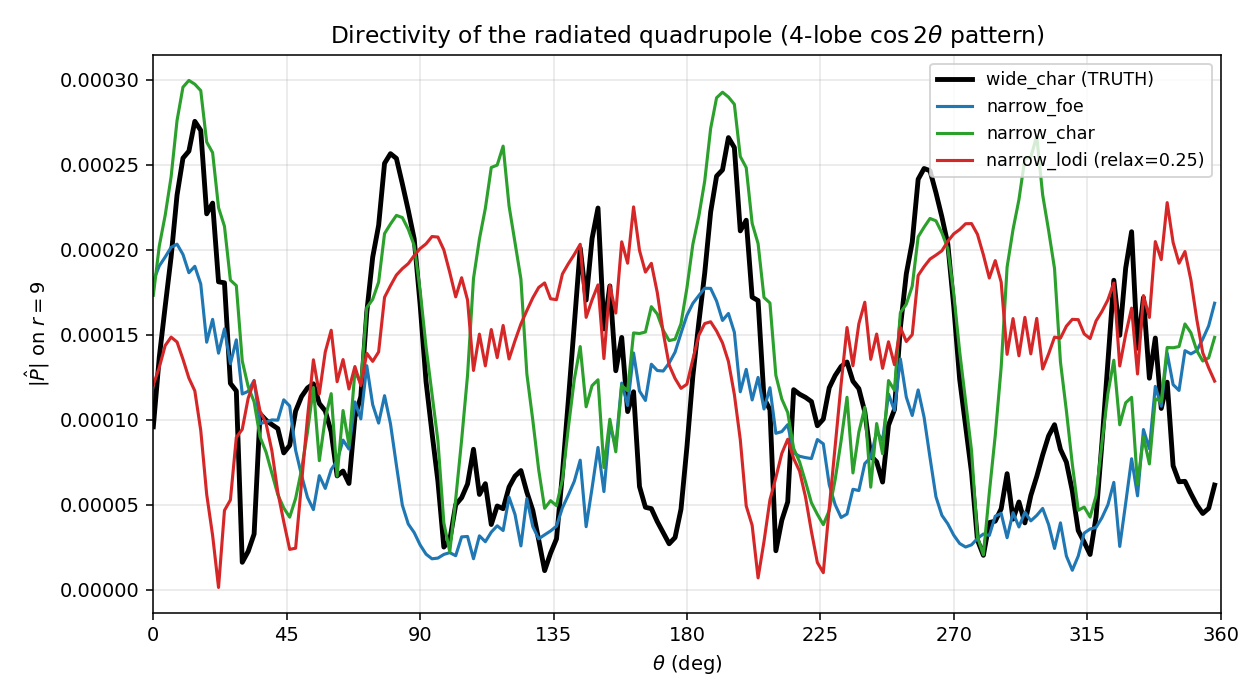
\includegraphics[width=0.8\textwidth]{figures/cvp_directivity.png}
  \caption{Directivity $|\hat P|(\theta)$ on $r=9$. The trace is dominated by
  spiral-arm crossings and residual near field, not a clean $\cos2\theta$
  quadrupole lobe pattern, and the four closures trace curves of equal
  magnitude --- visual confirmation that the wave does not discriminate them.}
  \label{fig:dir}
\end{figure}

\subsection{Mean anchoring is the only clean discriminator}
The only field-level difference exceeding its noise is the DC mode --- the
far-field mean pressure, a weak ($<1\%$ of $p_0$) effect. Over the window the
annulus-mean drift is $-8\times10^{-5}$ (\textit{foextrap}) $\approx
+1.4\times10^{-4}$ (characteristic) $\ll +7.2\times10^{-3}$ (LODI), and the
absolute far-field mean offset is smallest for the characteristic closure (close
to the wide truth), then \textit{foextrap}, then LODI. This reproduces the 1-D
trade-off and settles the fair-LODI question: a finite relaxation
$\sigma_p=0.25$ does \emph{not} win on the wave (it is the noisiest) and
under-anchors the mean (largest residual drift). Its advertised ``low reflection
plus anchoring'' is not realised here, because at near-normal incidence
\textit{foextrap} is already non-reflecting and the corrected characteristic
anchors the mean as well, without a relaxation term. The co-rotating vortex pair
is, in short, a clean \emph{negative control}.

\section{The decisive case: oblique strong-shock crossing}\label{sec:cylinder}
Where, then, does the characteristic closure earn its place? The answer is the
regime the 1-D and 2-D tests cannot probe: an oblique \emph{strong shock}
crossing a near lateral boundary. We test it on a supersonic cylinder
($M_\infty=1.7$, $\gamma=1.4$, WENO-Z, one AMR level), holding everything fixed
but the lateral BC code and progressively narrowing the lateral half-width.
Cold-started, the bow shock and near field establish by $t=30$; we measure the
centreline shock stand-off $\Delta x_s$ and the freestream density $\rhoinf$ at
the upstream edge.

\begin{figure}
  \centering
  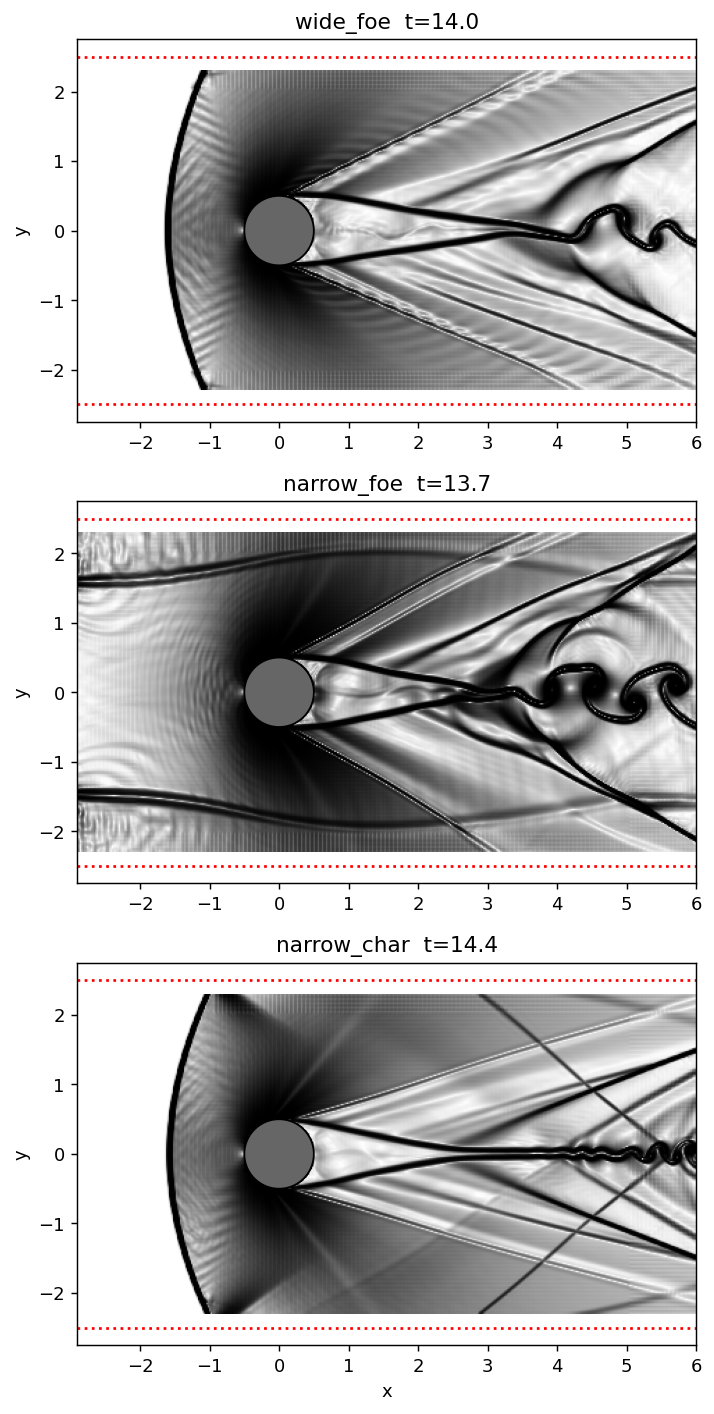
\includegraphics[height=0.82\textheight]{figures/schlieren_3way_narrow.png}
  \caption{Numerical schlieren at a narrow lateral half-width (panels top to
  bottom). The wide baseline (top) and the corrected characteristic closure at
  narrow width (bottom) carry an identical bow shock; narrow \textit{foextrap}
  (middle) admits a corrupted upstream state ($\rhoinf$ too high by
  $2.2\times$) and the bow shock is destroyed.}
  \label{fig:sch3}
\end{figure}

Figure~\ref{fig:sch3} tells the story at a glance. With the characteristic
closure the narrow-domain bow shock is indistinguishable from the wide baseline;
with \textit{foextrap} the upstream field is corrupted to a post-shock state
($\rhoinf$ too high by a factor $2.2$) and the shock collapses. The reason is
geometric: where an \emph{oblique} strong shock crosses the boundary,
\textit{foextrap}'s zero-gradient extrapolation cannot represent the jump and
feeds back a wrong state, whereas the characteristic closure \eqref{eq:fix}
correctly anchors the incoming invariant to the (supersonic) freestream.

\begin{figure}
  \centering
  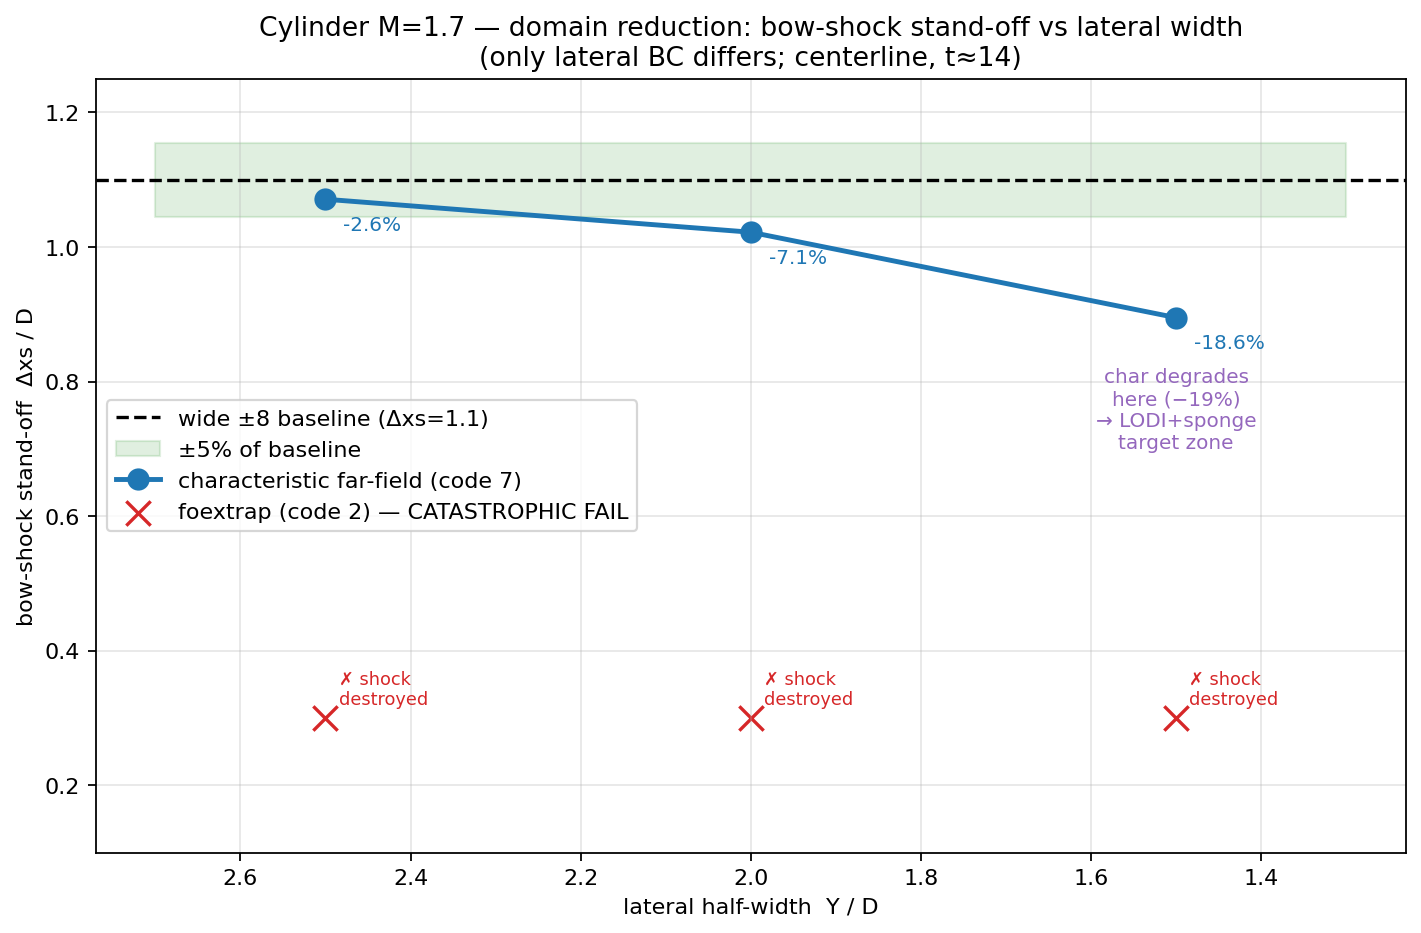
\includegraphics[width=0.8\textwidth]{figures/standoff_vs_width.png}
  \caption{Bow-shock stand-off $\Delta x_s$ versus lateral half-width (baseline
  wide $\pm8$, $\Delta x_s=1.10D$). The corrected characteristic closure (code
  7) drifts only gradually as the boundary closes in and never fails;
  \textit{foextrap} (code 2) is catastrophic at every narrow width.}
  \label{fig:standoff}
\end{figure}

Figure~\ref{fig:standoff} quantifies the gain. Taking the wide $\pm8$ stand-off
$\Delta x_s=1.10D$ as baseline, the characteristic closure preserves it to
$-2.6\%$ at $\pm2.5$, $-7.1\%$ at $\pm2.0$ and $-18.6\%$ at $\pm1.5$, with the
freestream density and post-shock ratio correct at all widths --- a graceful
degradation, never a failure. \textit{foextrap} is catastrophic at every narrow
width. The corrected characteristic closure therefore enables a $\sim2.5\times$
lateral-domain reduction ($\pm5\to\pm2.0$) with the shock stand-off held to
$7\%$, a regime in which \textit{foextrap} is simply unusable. This --- not free
radiation --- is where a characteristic far-field is decisive.

\section{Conclusions}\label{sec:concl}
Three controlled experiments, of increasing dimensionality, give a consistent
picture of far-field boundary conditions for compressible immersed-boundary
flow.
\begin{enumerate}
\item The solver's as-shipped algebraic ``NSCBC'' reflected $78\%$ of a
normally incident acoustic wave. This is exactly the $\sigma\to\infty$ limit of
a relaxed characteristic condition (it hard-pins the back-pressure), not a bug.
A one-line correction \eqref{eq:fix} --- impose the incoming Riemann invariant
from the freestream rather than the pressure --- restores $R<10^{-5}$ while
keeping the mean-state anchoring that \textit{foextrap} lacks.
\item For genuine free radiation (the co-rotating vortex pair), a rigorous
drift-free, phase-aware, floor-calibrated metric shows that \emph{no} closure
beats simple extrapolation on the wave: every closure's corruption of the
radiated quadrupole lies below the truth-against-itself noise floor. The only
field that discriminates the closures is the mean pressure, and even there the
effect is below $1\%$ of $p_0$. A finite-relaxation LODI does not improve on
this --- it is the noisiest on the wave and the weakest at anchoring.
\item The characteristic closure is decisive in one regime the wave tests cannot
probe: an oblique strong shock crossing a near boundary. There it enables a
$2.5\times$ domain reduction with the bow-shock stand-off preserved to $7\%$,
whereas \textit{foextrap} catastrophically corrupts the upstream field.
\end{enumerate}
The practical recommendation follows. On supersonic streamwise faces all
closures coincide and are exact. On lateral far fields that no strong shock
crosses, \textit{foextrap} is the simplest sound choice (non-reflecting at
near-normal incidence, passes entropy and vorticity, mean anchored by the
supersonic inflow). Where the domain must be narrowed until a bow shock crosses
the lateral boundary, the corrected characteristic closure \eqref{eq:fix} is
required. Boundary-condition quality for compressible external flow is governed
by mean-state anchoring and shock crossing --- not by free-wave reflection,
which is the property the non-reflecting-BC literature most often emphasises.

\begin{acknowledgements}
Computations were performed on the project HPC allocation. The author thanks the
reviewers of the internal validation campaign.
\end{acknowledgements}

\noindent\textbf{Declaration of interests.} The author reports no conflict of
interest.

\begin{thebibliography}{}

\bibitem[Colonius(2004)]{colonius2004}
Colonius, T. 2004 Modeling artificial boundary conditions for compressible flow.
\textit{Annu. Rev. Fluid Mech.} \textbf{36}, 315--345.

\bibitem[Lodato \textit{et~al.}(2008)]{lodato2008}
Lodato, G., Domingo, P. \& Vervisch, L. 2008 Three-dimensional boundary
conditions for direct and large-eddy simulation of compressible viscous flows.
\textit{J. Comput. Phys.} \textbf{227}, 5105--5143.

\bibitem[Mitchell \textit{et~al.}(1995)]{mitchell1995}
Mitchell, B. E., Lele, S. K. \& Moin, P. 1995 Direct computation of the sound
from a compressible co-rotating vortex pair. \textit{J. Fluid Mech.}
\textbf{285}, 181--202.

\bibitem[Motheau \textit{et~al.}(2017)]{motheau2017}
Motheau, E., Almgren, A. \& Bell, J. B. 2017 Navier--Stokes characteristic
boundary conditions using ghost cells. \textit{AIAA J.} \textbf{55} (10),
3399--3408.

\bibitem[Poinsot \& Lele(1992)]{poinsot1992}
Poinsot, T. J. \& Lele, S. K. 1992 Boundary conditions for direct simulations of
compressible viscous flows. \textit{J. Comput. Phys.} \textbf{101}, 104--129.

\bibitem[Rudy \& Strikwerda(1980)]{rudy1980}
Rudy, D. H. \& Strikwerda, J. C. 1980 A nonreflecting outflow boundary condition
for subsonic Navier--Stokes calculations. \textit{J. Comput. Phys.}
\textbf{36}, 55--70.

\bibitem[Thompson(1987)]{thompson1987}
Thompson, K. W. 1987 Time dependent boundary conditions for hyperbolic systems.
\textit{J. Comput. Phys.} \textbf{68}, 1--24.

\bibitem[Yoo \& Im(2007)]{yoo2007}
Yoo, C. S. \& Im, H. G. 2007 Characteristic boundary conditions for simulations
of compressible reacting flows with multi-dimensional, viscous and reaction
effects. \textit{Combust. Theory Model.} \textbf{11} (2), 259--286.

\end{thebibliography}

\end{document}
